\section{模型设计及实现}

% 5 页

在这一节,本文将对 BGP 路由中的异常检测问题的本质进行探讨,并对其做出公式化的推理,通过一种新颖的方式将其转化为另一种基于随机游走的路径的问题。为了验证上述思路的正确性,本研究还据此实现了一种多步异常检测模型,它的基本结构如图 \ref{c5-model} 所示,主要由采样、嵌入、聚合和异常检测部分组成。

\begin{figure}[h]
    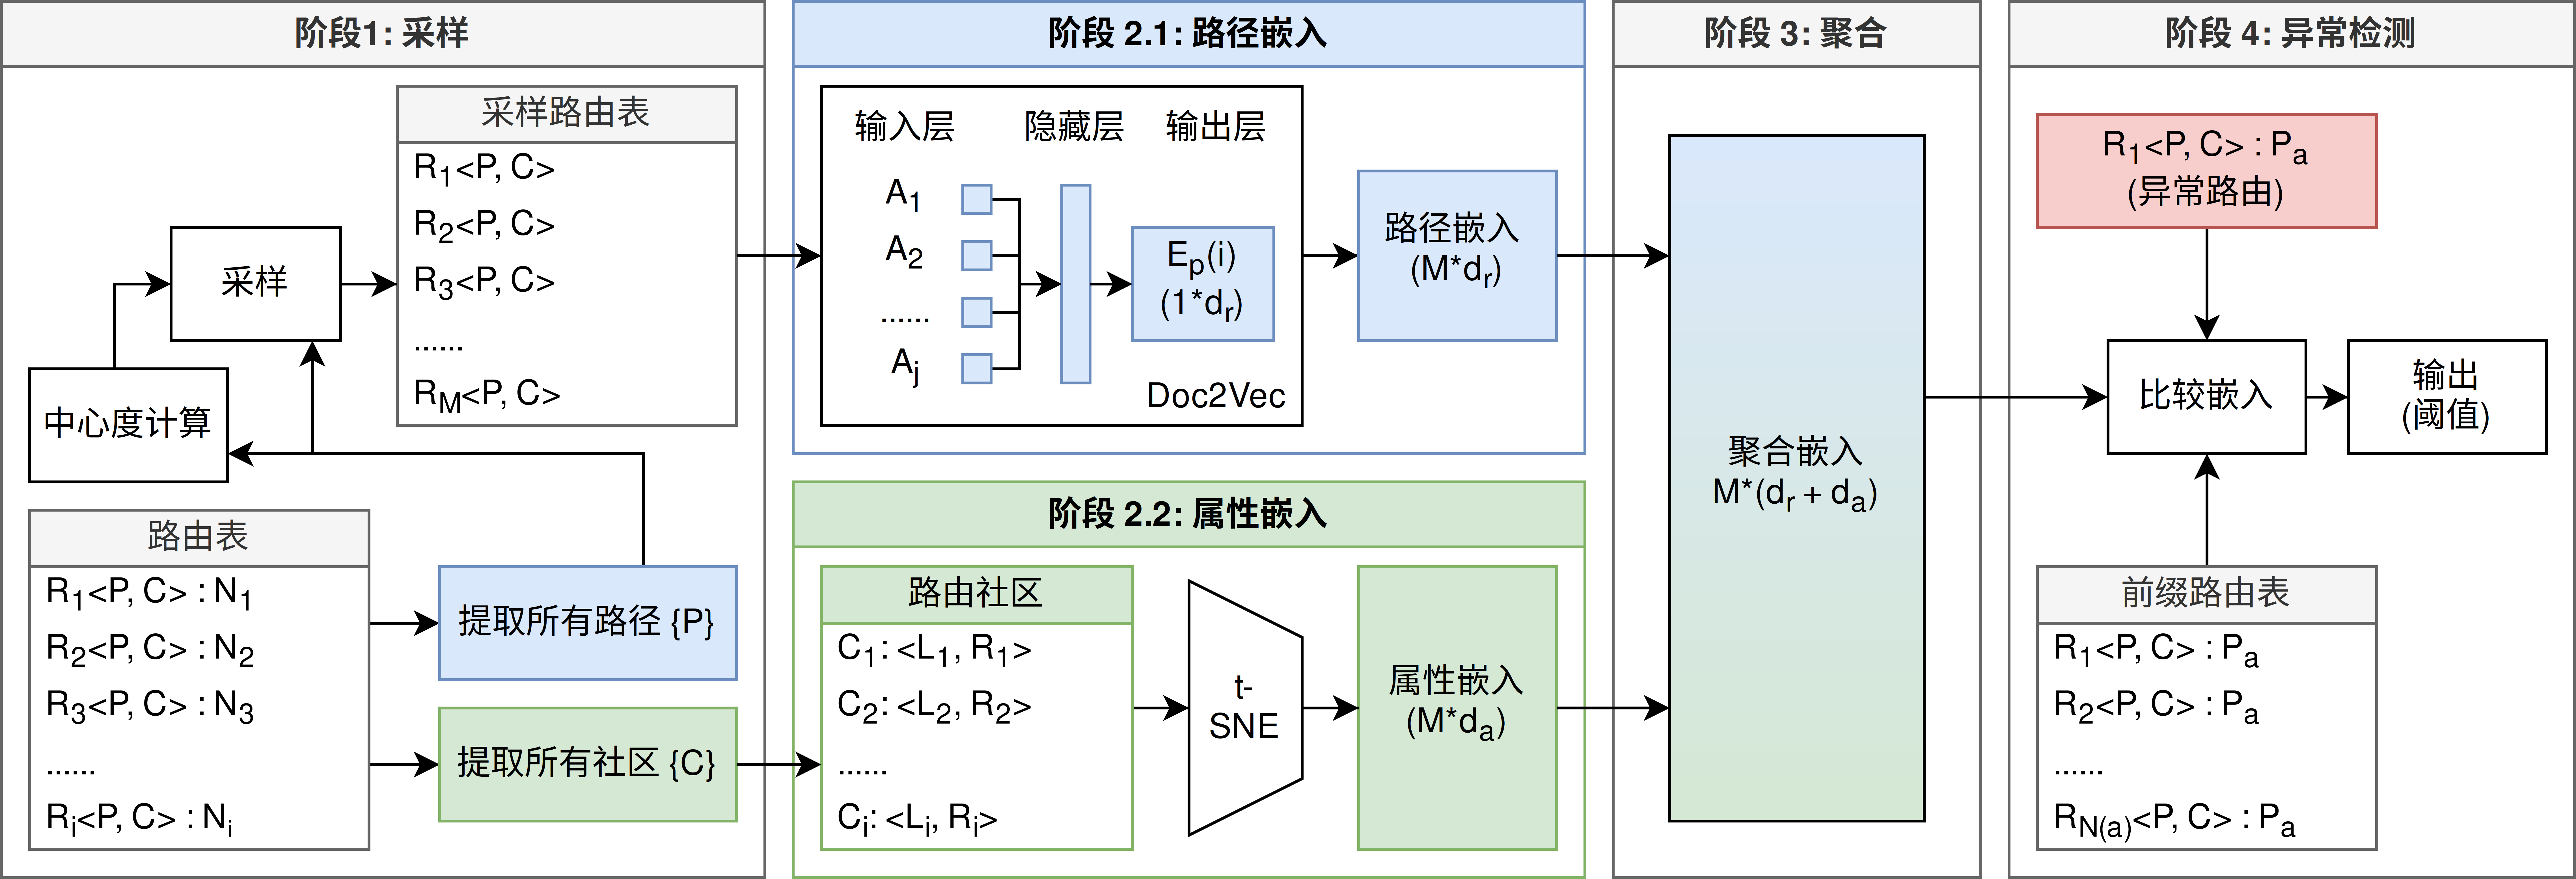
\includegraphics[width=\linewidth]{chapter/c5_images/c5_model.png}
    \caption{模型结构图}
    \label{c5-model}
\end{figure}

\begin{enumerate}
    \item 采样模块反映了本节研究的核心观点,使用了一种新颖的方式采样路由路径,并分离其中的拓扑和属性特征。
    \item 路径嵌入模块对采样后的、符合随机游走的统计学特征的路径集进行学习并获得对应的嵌入向量。
    \item 属性嵌入模块则是根据路由的社区属性,对其进行降维处理,获得社区属性对应的嵌入向量。
    \item 聚合模块将二者结合起来,作为最终的嵌入信息。
    \item 异常检测模块使用基于嵌入误差的方法对路由更新进行相似度计算,给出异常检测分数结果,并可选地根据阈值判断路由异常。
\end{enumerate}

\subsection{基于路由度量信息的样本采样}

这是模型的第一部分,它利用了随机游走的思想,将数据视作为随机游走的等效结果,通过一种等效化采样的方法处理原始数据,使其分布满足一种特定的基于最短路权重的随机游走采样方法,以便于后续通过基于随机游走的图网络嵌入进行异常检测任务。

\subsubsection{图上的随机游走}

本步骤的核心观点在于,将路由数据集中的路由条目的自治系统路径属性与在图上进行随机游走后产生的路径相关联起来。为了实现并验证这一目标,需要对网络拓扑上的数据集采集方法的特点进行分析。

边界路由协议在一般情况下,对路由选择的影响反映在自治系统路径和社区属性上\citing{feamster2004model},它们共同作用决定某个网络将以何种路径被抵达。由于不同运营商的社区属性定义一般是不一样的,此类信息仅能作为一种拓扑无关的特征使用,本文在随机游走性质的研究主要体现在自治系统路径,即拓扑信息上。

在路由表中宣告的每一个地址块 B 都对应着至少一个可访问的网络,以及至少一条路由条目 $\{R_1, R_2, ... R_n\}$。根据本章前一节的分析,路由表$\{B_1,...B_m\}$中的每个地址块所涉及到的路由则可以理解为一种随机游走策略:以数据包的视角而言,随机游走路径实质上是从随机的采集点$\{A\in{A_1, A_2...}\}$出发,经过 $m \times n$ 轮采样到达地址块源网络的路径集合。

因为它是一种有效的随机游走采样方法,只要输入的数据满足这样的条件,就可以对路由进行进一步的嵌入,进而进行异常检测。

\subsubsection{基于随机游走介数中心度的路径采样}

由于广域网络的路由选择模型是通过最短路径实现的,对这样的数据构图更适合介数中心度指标。然而,实际的路由数据集中的数据并不是最短路径,不同的自治系统和基于 BGP Add-Path (RFC5492)\citing{walton2016advertisement}的路由收集会话都会发送同一网络的不同前缀的次优路由,在此场景下,传统的介数中心度指标会受到此类因素的干扰,与实际拓扑对应的值存在偏差,因此基于随机路径的数据需要一种新的度量方式。由于上述原因,为了更好地度量在非最优路径集合内,某一节点对网络的影响力,本研究引入了随机游走介数中心度这一度量单位。

如公式\ref{betweeness}所示,通常情况下的介数中心度被定义为一个节点作为两个其他节点之间最短路径上的桥梁的次数。
\begin{equation} \label{betweeness}
C_{betweenness}(v) = \Sigma_{s \neq v \neq t \in V}\frac{\sigma_{st}(v)}{\sigma_{st}}
\end{equation}
根据此公式,对于图中的每一对顶点 $s,t \in V$,计算它们之间的最短路径$\sigma_{st}$,随后对每一个顶点计算通过该顶点的最短路径$\sigma_{st}(v)$的加权和。

而数据集中的路由显然不满足这一条件,它包含不同位置、不同网络、不同发送策略的路由,因而将使用“不那么最短路径”的度量来衡量它的介数中心度。

由于 BGP 路由在一般情况下遵循最短自治系统路径原则,并且大部分 BGP 劫持都是通过宣告更短自治系统路径的路由进行的,路由表中的路由条目中的路径部分 $P$ 显然在一定程度上是通过在真实的网络拓扑 $G \left\langle V,E \right\rangle$ 下使用某种基于随机游走的介数中心度的方法进行采样的结果路径集合。

Newman 提出了一种对随机游走进行中心度度量的方法,它被称为随机游走介数中心度。\citing{agryzkov2014new} \citing{newman2005measure} 该度量单位以公式\ref{rw_betweeness}的方式被定义。
\begin{equation} \label{rw_betweeness}
C_{RWbetweenness}(v) = \Sigma_{s \neq v \neq t \in V}\ p_{st}(v)
\end{equation}
该公式去除了最短路径的条件,从而计算路径集合内每一条可行的路径中,经过点$v$路径的加权和,在本研究中,连通$s,t$路径的全集即为路由数据集中以$s,t$分别作为起始和结束节点的自治系统路径。

有了上述前提,问题的目标现在被转化为,在已知部分路由信息 $R_o$ 的条件下,进行二次采样 $M‘$,使得采样的结果与在 G<V,E> 上进行加权随机游走 $M_r$ 的结果一致,即 $M_r(G<V,E>) = M'(M(G<V,E>)) = M'(R_o)$ ,对新的路由更新信息 $R_update$ 做出异常检测。

模型需要先根据给定路径 $R_o$ 计算出各个节点的随机游走介数中心度,并据此采样出 $m'(R_o) \in R_o$。

值得注意的是,网络路由数据集大多是由配置了路由反馈会话的路由器向收集器发送全部或者部分路由,并不遵循以随机游走介数中心度为权重进行随机游走的采样规则,因此需要使用以下的采样方法来使处理后的数据集达到期望的分布。

此处规定等价采样 $M'$ 的输入是包含若干网络 $\{N1,N2,...N_{N_{prefix}}\}$ 的路由表,$M'$ 将对输入中的每个 N 中的路由项 R 进行采样,使得 $j < i$。

具体来讲,对于每一个网络路由 $N_i$,模型对其包含的路由的路径子集 $\{P_1, P_2, P_3, ... P_{n_{route}(i)}\}, R_i<P_i, C_i> \in N_i $ 进行随机游走介数中心度的计算,得到一个节点与中心度的映射 $A_i \rightarrow C_{RWbetweenness}(A_i)$,随后以公式\ref{omega_p}规定路径的采样权重为它路径上的平均中心度:
\begin{equation} \label{omega_p}
\omega_p(P_i) = \frac{\sum_{A_i \in P_i}^{len(P_i)} C_{RWbetweenness}(A_i) + \theta}{len(P_i)}
\end{equation}

最终的采样结果使用 $R_{sampled} = top(k, R_o)$,$\theta$ 在这里起到了控制路径长度的作用,当 $\theta \gg \sum C_{RWbetweenness}(A_i) $ 时,可以近似的认为是完全以路径长度作为度量进行采样。

\subsection{路由路径与特征嵌入}

\subsubsection{基于 Doc2Vec 的路由拓扑嵌入}

在这一阶段,模型将以路径作为模块的输入,使用模型捕获路径中的拓扑关系,输出对应的嵌入。本文将先从 Node2Vec 出发探讨这一可能性,随后介绍本模型实际使用的 Doc2Vec 方法\citing{le2014distributed}。

对于传统的随机游走嵌入模型,通常的方法是使用 Node2Vec 来从采样后的路径中获得节点的嵌入\citing{grover2016node2vec},然而,由于 Node2Vec 仅能够对单个节点进行表征,无法对路径及其属性进行建模,因此需要将其进行拓展。

Doc2Vec 是一种从可变长序列(通常是文字)中提取嵌入特征的方法\citing{le2014distributed},它能够通过提取序列间元素的关系,直接对整个序列生成特征向量。

正如节点 V 能够与词语表征相对应,采样路径 P 也能够与段落表征相对应,这与 node2vec 和 word2vec 的对应关系类似。通过基于 Doc2Vec 的 path2vec 模型,能够更好地捕获路径中节点间的关联,即路由每一跳之间的联系,将采样路径转换为嵌入向量。

Doc2Vec 模型存在两种不同的训练方法,分别称为 DM(Distributed Memory)和 DBOW(Distributed bag of words)\citing{murdock2014learning}。对于本文所涉及到的问题而言,Distributed Memory 方式获得的向量能够作为输入序列的上下文,因而更适合在此场景中使用。

因此,本文将路径列表使用 Distributed Memory 方法放入 Doc2Vec 模型中进行训练,然后对每个路径输出一个 $d_r$ 长度的向量作为路径的表征。

\begin{figure}[h]
    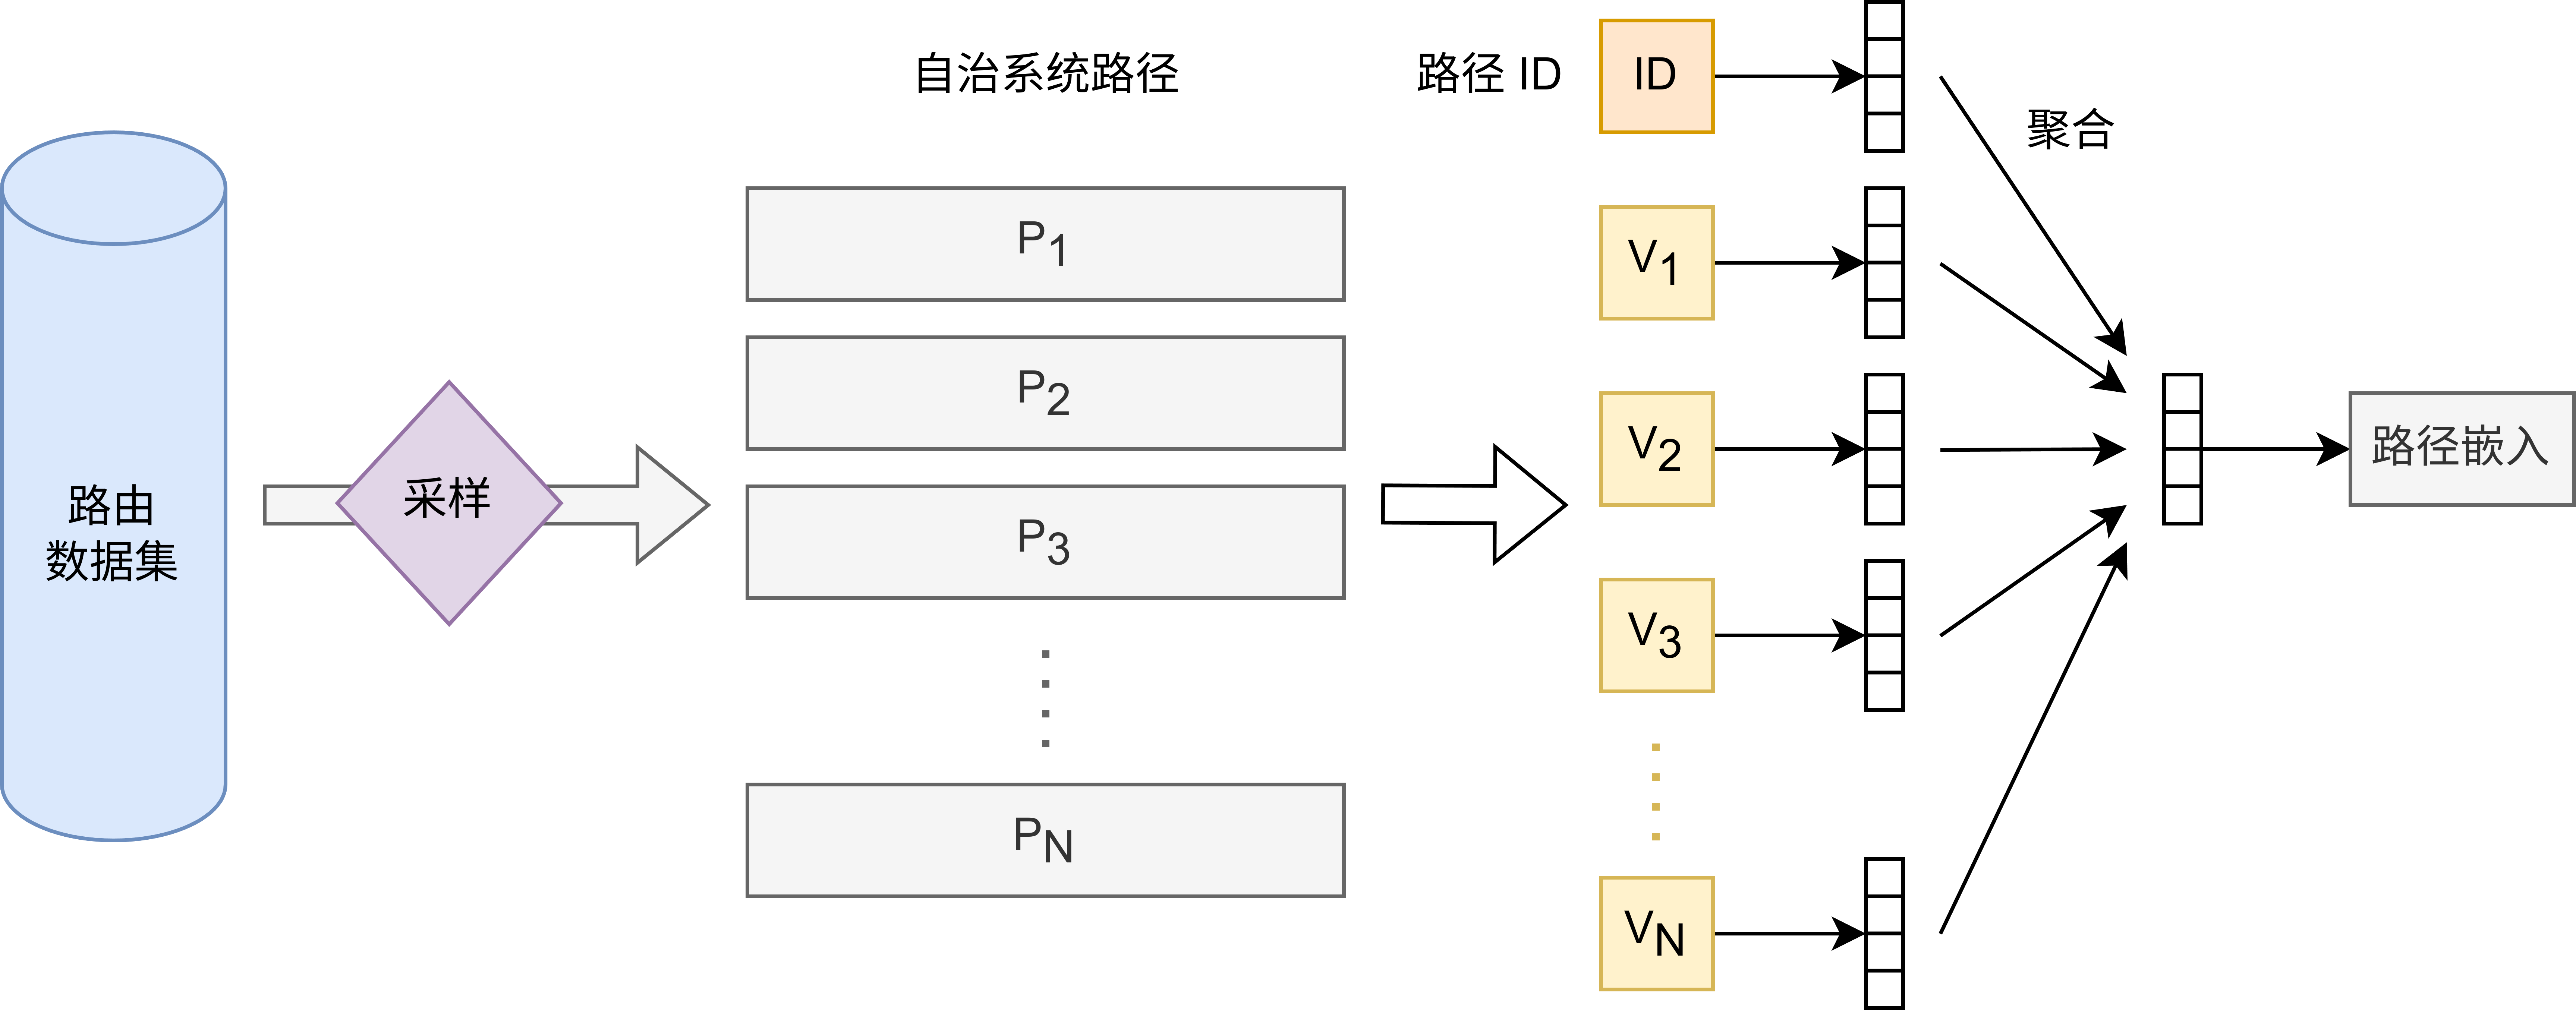
\includegraphics[width=0.9\linewidth]{chapter/c5_images/c5_model-dm.png}
    \caption{使用 Distributed Memory 方法训练路径嵌入}
    \label{c5_model-dm}
\end{figure}

% 图

如图 \ref{c5_model-dm} 所示,在模型中,每一个路径都被赋予一个唯一的 ID,并将其映射到矩阵 D 的其中一列以表示上下文信息,在此之后,路径中的每一个节点都将被映射到矩阵 W 中的其中一列,它们共同被输入 Doc2Vec 模型中,通过 Distributed Memory 方法转换为一列嵌入向量,从而被用于下游的异常检测任务。

\subsubsection{基于 t-SNE 的路由属性嵌入}

在路径拓扑进行嵌入之外,另一个模块是对路径的属性进行嵌入表示,由于 Community 属性并不包含特定的拓扑信息,在不同网路中定义方式也差异很大,模型在这里直接将 Community 映射到一个特定的 one-hot 向量,然后通过 t-SNE 对数据进行降维\citing{van2008visualizing},将其输出为 $d_a$ 长度的向量作为特征的表征。

\subsection{特征的聚合和异常检测}

由于前面两个模块分别输出路径的拓扑和属性两个方面的嵌入,这一模块目的是将其结合起来作为最终的嵌入向量用作后续的异常检测。

对于异常检测而言,只需对新的路由 $R_{update}$ 进行一次嵌入计算,然后将其与现有的对应路由 $R_{exist} \in R$ 进行相似度对比,偏移过大的路由条目将作为异常路由输出。

具体的相似度计算使用如公式\ref{s5_cos_dist}所述的余弦相似度方法:
\begin{equation} \label{s5_cos_dist}
D_{cos}(A,B) = 1 - \frac{\sum_{i=1}^{d_r+d_a} A_i B_i}{\sqrt{\sum_{i=1}^{d_r+d_a} A_i^2}\sqrt{\sum_{i=1}^{d_r+d_a} B_i^2}}
\end{equation}